\documentclass[UTF8]{ctexart}
\usepackage{CJKutf8}
\usepackage{graphicx}
\usepackage{amsmath}
\usepackage{diagbox}
\usepackage{hyperref}
\usepackage{xcolor}
\usepackage{cite}
\usepackage{indentfirst}
  \author{黄晃 数院 1701210098 }
  \title{大数据中的算法项目一}
\begin{document}
\bibliographystyle{plain}
\bibliography{1}
  \maketitle
  \section{问题一}
  原问题为
  \begin{equation}\label{p:1}
    \begin{split}
       min\  &  \|x\|_{1} \\
       sub\  &  Ax = b\\
    \end{split}
  \end{equation}
  \subsection{cvx calling mosek or gurobi}
  因为primal~\ref{p:1}是个凸问题,cvx下可以直接
  $$minimize(norm(x,1))$$
  $$sub Ax=b$$
  \subsection{calling mosek or gurobi directly}
  \subsubsection{问题转化}
  将primal转化为LP
        \begin{equation}\label{p:2}
    \begin{split}
    min\  &  \Sigma_{i=1}^{n}t_{i} \\
    sub\  & -t_{i} \leq x_{i}\leq t_{i}
    \end{split}
  \end{equation}
  引入$v_{i}=t_{i}-x_{i}$,则~\ref{p:2}转化为
      \begin{equation}\label{p:3}
    \begin{split}
    min\  &  \Sigma_{i=1}^{n}(x_{i}+v_{i}) \\
    sub\  & 2x_{i}+v_{i} \geq 0 \\
            & v_{i} \geq 0
    \end{split}
  \end{equation}

  \subsection{bregman iteration}
   Classical Augmented Lagrangian method (or Bregman method), where each augmented Lagrangian function is minimized by using the proximal gradient method
   \subsubsection{外部迭代}
   由所给参考文献,我们选择所给的Bregman method中的version2:
         \begin{equation}
    \begin{split}
    b_0=0, x_0=0 \\
    for k = 1,2,3,\cdots do \\
    b_{k+1} = b + b_k - Ax_k \\
    x_{k+1} = argmin\ \mu \|x\|_1 + \frac{1}{2}\|Ax-b_{k+1}\|^2
    \end{split}
  \end{equation}
  \subsubsection{子问题}
  更新$x_k$时,我们使用要求的proximal方法,所以子问题的迭代为
  $$
  x_{ m+1}=shrink(x_m-\tau \nabla f(x),\mu \tau)
  $$
  其中$f(x)=\frac{1}{2}\|Ax-b_{k+1}\|^2$,k为外部迭代次数,m为内迭代次数
  \paragraph{子问题终止条件}
  子问题通过$\|x_{m+1}-x_m\|<\epsilon\ or\ m > MAX$来终止
  \paragraph{同伦}
  为了更好的求解子问题,对于给定的$\mu_0$,采取了同伦的技巧来进行优化,具体为依次求解$\mu =10000\mu,1000\mu,100\mu,10\mu,\mu$对应的问题,然后用其解作为下一次的初始点,相应的终止条件$\epsilon$也做适当放大
  \paragraph{子问题参数}
  参数$\tau = \frac{1}{norm(A^TA)}\mu,\epsilon= [2e-4,1e-5,2e-6,1e-6,1e-6]$
  \subsubsection{外部终止条件以及参数的选择}
  根据文献,外部迭代的终止条件为
  $$
  \frac{\|b_k-Ax_k\|}{\|b\|}<1e-8
  $$
  \paragraph{}
  参数$\mu_0=0.001$



  \subsection{ADMM for dual}
   Alternating direction method of multipliers (ADMM) for the dual problem
   \subsubsection{外部迭代}
    对偶问题为
  \begin{equation}\label{p:3}
    \begin{split}
       max\  &  b^Ty \\
       sub\  &  \|A^Ty\|_\infty \leq 1\\
    \end{split}
  \end{equation}
由参考文献,ADMM迭代格式为
  \begin{equation}
    \begin{split}
       z_{k+1} = &  P_{B_1^\infty}(A^Ty_k+x_k/\beta) \\
       y_{k+1} = &  (A^TA)^{-1}(Az_{k+1}-(Ax_k-b)/\beta)\\
       x_{k+1} = &  x_k - \gamma \beta (z_{k+1}-A^Ty_{k+1})
    \end{split}
  \end{equation}
\subsubsection{终止条件以及参数的选择}
根据文献,终止条件为
$$
min\{ \|r_p\| / \|b\|, \|r_d\| / \sqrt{m}, | \triangle | / \|x\|_1\} \leq \epsilon
$$
其中
  \begin{equation}
    \begin{split}
       r_p = &  Ax-b \\
       r_d = &  A^Ty-z\\
       \triangle = & b^Ty-\|x\|_1\\
    \end{split}
  \end{equation}
  \paragraph{}
  参数$\gamma=1,\beta=2*m/\|b\|_1,\epsilon=1e-8$

  \subsection{数值结果}
%  \begin{table}
%  \centering
%  \caption{问题一}
\begin{tabular}{|r|r|r|r|r|}
\hline
method & nrm1fun & res  & cpu & err to mosek\\ \hline
cvx-mosek &         7.85e+01&  1.90e-10& 1.38 & 0 \\
 cvx-gurobi &7.85e+01& 2.95e-09&  0.86& 3.29e-10  \\
call-mosek & 7.85e+01 & 1.62e-07&  1.90& 1.00e-09 \\
call-mosek&  7.85e+01& 1.62e-07& 1.92& 1.00e-09 \\
bregman& 7.85e+01& 3.95e-07&  3.25& 2.43e-09 \\
admm&  7.85e+01& 4.49e-13&  0.07& 3.60e-09 \\
\hline
\end{tabular}
%   \end{table}
\subsubsection{结果分析}
\begin{itemize}
  \item 各个算法都达到了1e-9的精度
  \item 约束条件$Ax=b$的残量都达到了1e-7以上
  \item cpu时间方面,除了ADMM外均与cvx处在一个量级
  \item ADMM除了耗时极短(0.07)外,约束条件也满足的最好,达到了1e-13,高于cvx的1e-10
\end{itemize}
  \section{问题二}

  Algorithms For Sparse Inverse Covariance Estimation
    \subsection{数据产生}
  由参考文献,$S=\Sigma_n=\frac{1}{n}\sum_{k=1}^{n}(X_i-\overline{X})(X_i-\overline{X})^T$,其中$\overline{X}=\frac{k=1}{n}X_k$.
  $X\sim N(0,\Sigma_0),\Sigma_0=\Omega_1^{-1}$,所要求的两个模型只有$\Omega_0=(\omega_{ij})$不同.
  生成$\Omega_0$后可得到对应的$\Sigma_0$,然后生成n=100组数据(X),然后求X的协方差矩阵作为$\Sigma_n$,
  注意到文献所给的定义与一般的定义有系数上的差别,所以用matlab的cov函数求得协方差后还需乘以$\frac{n}{n-1}$
  \subsubsection{model1}
  $\omega_{ij}=0.6^{|i-j|}$
  \subsubsection{model2}
  $\Omega_0=B+\delta I$,其中B非对角元满足两点分布,以0.1概率为0.5,0.9概率为0.然后$\delta$使得$\Omega_0$的条件数等于p,最后再单位化对角元.
  \paragraph{$\delta$的确定}
  要使得$\sigma_1/\sigma_p=p$,先求B最大特征与最小特征$\lambda_1,\lambda_p$,然后由于$\Omega$的奇异值满足$\sigma_k=abs(\lambda_k+\delta)$,所以取$\delta=\frac{p\lambda_p-\lambda_1}{1-p}$即可

  \subsection{1}
    \begin{equation}
    \begin{split}
    \max_{X\succeq0} logdet(X)-Tr(SX)-\rho \|X\|_1
    \end{split}
  \end{equation}
  其中
      \begin{equation}
    \begin{split}
\|X\|_1=\sum_{ij}|X_{ij}|
    \end{split}
  \end{equation}
    \subsubsection{dual}
    注意到
          \begin{equation}
    \begin{split}
\|X\|_1=\sum_{ij}|X_{ij}|=\max_{\|U\|_{\infty}\leq1}Tr(UX)
    \end{split}
  \end{equation}
  而
      \begin{equation}
    \begin{split}
   & \max_{X\succeq0} logdet(X)-Tr(SX)-\rho \|X\|_1  \\
    = &\max_{X\succeq0}\min_{\|U\|_{\infty}\leq1} logdet(X)-Tr(SX)-\rho Tr(UX)\\
    = & \max_{X\succeq0}\min_{\|U\|_{\infty}\leq\rho} logdet(X)-Tr(SX)- Tr(UX)\\
    = & \max_{X\succeq0}\min_{\|U\|_{\infty}\leq\rho} logdet(X)-Tr((S+U)X)\\
    \end{split}
  \end{equation}
交换max与min,对X求导$D(X)=X^{-1}-U-S$,由一阶条件,对偶函数为
\begin{equation}
    \begin{split}
        g(U)  = & \min_{\|U\|_{\infty}\leq\rho}\max_{X\succ0} logdet(X)-Tr((S+U)X)\\
    = & \min_{\|U\|_{\infty}\leq\rho}-logdet(U+S)-p
    \end{split}
  \end{equation}
  等价于
      \begin{equation}
    \begin{split}
    \min_{U\in S_{+}}&-logdet(U+S)-p \\
    sub & \|U\|_{\infty}\leq\rho\\
    \end{split}
  \end{equation}
  \subsubsection{use cvx}
  只用考虑$\|X\|_1$的表示即可,这里选择构造全一矩阵$S1$,则$\|X\|_1=trace(S1*abs(X))$
\subsubsection{method}
选择了~\cite{NIPS2012_4574}所描述的threating算法来求解该问题,详细见~\cite{NIPS2012_4574}的3.2节,在此不再赘述
\paragraph{初值}
初值选择参考~\cite{NIPS2012_4574},$X_{ii}=(S_{ii}+\rho)^{-1}$
\paragraph{终止条件}
终止条件为对偶间隙$\delta<\epsilon$,或者达到最大步数,或者是对给定的下降方向,线搜索找不到满足要求的$\alpha$
\subsubsection{数值结果}
为了比较算法与cvx的计算结果,定义如下两个量
$$
err_F = (F(X_2) - F(X_1))/(1+abs(F(X_1)))
$$
$$
err_X = norm(X_2-X_1)/(1+norm(X1))
$$
其中$X_1,X_2$分别为cvx与threating的解

$F(X)=-logdet(X)+trace(SX)+\rho \|X\|_1$为目标函数
\begin{table}
  \centering
  \caption{model1}\label{table:1}
\begin{tabular}{|c|c|c|c|c|c|c|c|}
  \hline
  % after \\: \hline or \cline{col1-col2} \cline{col3-col4} ...
  \diagbox{$\rho$}{method}& \multicolumn{2}{c|}{$cvx$} &\multicolumn{5}{c|}{threating}\\
  \hline
  &cpu&F &cpu& F& $err_F$ &$ err_X $&ite\\
  \hline
  10 & 2.02  & 1.05e+02 &  0.01 & 1.05e+02   &   3.07e-07 & 1.84e-05 & 1 \\
  1 & 2.67  & 6.63e+01 &  3.21 & 6.63e+01   &   -3.70e-07 & 2.88e-05 & 10000\\
  0.1&2.19  & 4.90e+01 &  8.43 & 4.90e+01   &   1.23e-07 & 4.65e-05  &10000\\
  0.01& 1.91  & 1.89e+02 & 41.92 & 1.89e+02   &   -2.84e-05 & 4.46e-05 & 10000\\
  0.001&1.86  & 5.95e+01 & 16.77 & 5.95e+01   &   -9.69e-06 & 8.18e-05 & 10000 \\
  \hline
\end{tabular}
\end{table}

\ref{table:1}\ref{table:2}分别展示了两个model的计算结果

此外为了观察终止条件的满足情况,下面图~\ref{fig:1}~\ref{fig:2}展示了两个model$\rho=0.001$时对偶间隙$\delta$随迭代的变化.
\begin{figure}[htbp]
\centering\includegraphics[width=3.5in]{1.eps}
\caption{model1}\label{fig:1}
\end{figure}


\begin{figure}[htbp]
\centering\includegraphics[width=3.5in]{2.eps}
\caption{model2}\label{fig:2}
\end{figure}

\begin{table}
  \centering
  \caption{model2}\label{table:2}
\begin{tabular}{|c|c|c|c|c|c|c|c|}
  \hline
  % after \\: \hline or \cline{col1-col2} \cline{col3-col4} ...
  \diagbox{$\rho$}{method}& \multicolumn{2}{c|}{$cvx$} &\multicolumn{5}{c|}{threating}\\
  \hline
  &cpu&F &cpu& F& $err_F$ &$ err_X $&ite\\
  \hline
  10 & 2.00  & 7.81e+01 &  0.01 & 7.81e+01   &   4.12e-06 & 2.50e-06 & 1 \\
  1  & 2.13  & 5.87e+01 &  0.00 & 5.87e+01   &   -5.85e-04 & 3.69e-02 & 1 \\    
  0.1 & 2.21  & 8.42e+01 & 30.11 & 8.42e+01   &   -3.46e-06 & 5.97e-05 & 10000 \\
  0.01 & 1.86  & 4.43e+01 & 26.10 & 4.43e+01   &   5.11e-06 & 1.02e-04 & 10000 \\
  0.001&1.56  & 3.26e+01 &  4.76 & 3.26e+01   &   1.90e-05 & 8.67e-04 & 10000 \\
  \hline
\end{tabular}
\end{table}

\subsubsection{结果分析}
\begin{itemize}
  \item 由于model1比model2形式更简单,显示在计算结果上就是threaing方法对model1处理的更好
  \item 观察到$\rho=10,1$时threating方法只进行了一次迭代,更换初值发现,这取决于初值的选择,更改为随机的一组初值,计算结果表现较差
  \item $\rho=0.1,0.01,0.001$时,threating方法均正常运行,迭代10000步计算结果均到了1e-4以上
  \item 预设的终止条件$\delta< \epsilon$在$\rho$较小时均为达到,具体见\ref{fig:1}\ref{fig:2}所示,在2000步左右趋于稳定,而不能达到预设的1e-4
  \item 时间方面,若只需达到表中所给精度,可将最大迭代次数改小至2000左右(因为对偶间隙条件达不到),所以threating方法的时间花费与cvx相当
\end{itemize}


\subsection{2(extra-credit)}
考虑问题
\begin{equation}
    \begin{split}
    \max_{X\succeq0}& \|X\|_1 \\
    sub& \|SX_I\|_1\leq \rho
    \end{split}
  \end{equation}
  \subsubsection{dual}
  定义集合$B=\{U\in S^p \mid U_{ij}\in \{1,-1\} \}$
  则有
  \begin{equation}
    \begin{split}
\|X\|_1=\sum_{ij}|X_{ij}|=\max_{\|U\|_{\infty}\leq1}Tr(UX)\\
    = & \max_{U\in B}Tr(UX)
    \end{split}
  \end{equation}
    则对应的lagrangian函数为
    $L(X,\Lambda)=\|X\|_1+\sum_{U_\alpha\in B}\lambda_\alpha(<U_\alpha,SX-I>-\rho)$
    一阶次梯度为
    $$\partial L/\partial X=Z+\sum_{U_\alpha\in B}\lambda_\alpha U_\alpha S$$,
    因为$Z_{ij}$可取遍$[-1,1]$,所以当且仅当$\|\sum_{U_\alpha\in B}\lambda_\alpha U_\alpha S\|_{\infty}\leq 1$时导数可取到0,而且易见此时取X=0可使次梯度为0.因此问题转化成
    \begin{equation}
    \begin{split}
    \min& \sum_{U_\alpha\in B}\lambda_\alpha + <\sum_{U_\alpha\in B}\lambda_\alpha U_\alpha>  \\
    sub& \|\sum_{U_\alpha\in B}\lambda_\alpha U_\alpha S\|_{\infty}\leq 1
    \end{split}
  \end{equation}
    \subsubsection{use cvx}
    类似于上一个问题,目标函数可写成trace(S1*abs(X)),而约束为$trace(S1*abs(S*X2-I)) <= rho$
  
    
  \end{document}
